\documentclass[10pt,journal,compsoc]{IEEEtran}
\usepackage[utf8]{inputenc}

% *** CITATION PACKAGES ***
%
\ifCLASSOPTIONcompsoc
  % The IEEE Computer Society needs nocompress option
  % requires cite.sty v4.0 or later (November 2003)
  \usepackage[nocompress]{cite}
\else
  % normal IEEE
  \usepackage{cite}
\fi
\usepackage{graphicx}
\usepackage{caption}
\usepackage{eurosym} 
\usepackage{array} 
\renewcommand{\tablename}{Tab.}
\graphicspath{ {images/} }
% *** GRAPHICS RELATED PACKAGES ***
%
\ifCLASSINFOpdf
  
\else
 
\fi
\newcommand\MYhyperrefoptions{bookmarks=true,bookmarksnumbered=true,
pdfpagemode={UseOutlines},plainpages=false,pdfpagelabels=true,
colorlinks=true,linkcolor={black},citecolor={black},urlcolor={black},
pdftitle={Bare Demo of IEEEtran.cls for Computer Society Journals},%<!CHANGE!
pdfsubject={Typesetting},%<!CHANGE!
pdfauthor={Michael D. Shell},%<!CHANGE!
pdfkeywords={Computer Society, IEEEtran, journal, LaTeX, paper,
             template}}%<^!CHANGE!

\hyphenation{op-tical net-works semi-conduc-tor}


\begin{document}

\title{Sistema domótico IoT basado en Raspberry Pi y control remoto por Telegram}
\author{Jesús Gómez Bellido}

% for Computer Society papers, we must declare the abstract and index terms
% PRIOR to the title within the \IEEEtitleabstractindextext IEEEtran
% command as these need to go into the title area created by \maketitle.
% As a general rule, do not put math, special symbols or citations
% in the abstract or keywords.
\IEEEtitleabstractindextext{%
\begin{abstract}
The abstract goes here.
\end{abstract}

% Note that keywords are not normally used for peerreview papers.
\begin{IEEEkeywords}
Computer Society, IEEE, IEEEtran, journal, \LaTeX, paper, template.
\end{IEEEkeywords}}


\maketitle


% To allow for easy dual compilation without having to reenter the
% abstract/keywords data, the \IEEEtitleabstractindextext text will
% not be used in maketitle, but will appear (i.e., to be "transported")
% here as \IEEEdisplaynontitleabstractindextext when compsoc mode
% is not selected <OR> if conference mode is selected - because compsoc
% conference papers position the abstract like regular (non-compsoc)
% papers do!
\IEEEdisplaynontitleabstractindextext
% \IEEEdisplaynontitleabstractindextext has no effect when using
% compsoc under a non-conference mode.


% For peer review papers, you can put extra information on the cover
% page as needed:
% \ifCLASSOPTIONpeerreview
% \begin{center} \bfseries EDICS Category: 3-BBND \end{center}
% \fi
%
% For peerreview papers, this IEEEtran command inserts a page break and
% creates the second title. It will be ignored for other modes.
\IEEEpeerreviewmaketitle

\section{Introduccion y objetivos}\label{sec:introduccion}

\IEEEPARstart En este Trabajo fin de Máster (TFM) vamos a tratar de ver el impacto 
que pueden generar las nuevas tecnologías que se están empezando a expandir.
Estas nuevas tecnologías tienen siempre en mente una perspectiva, el llamado
 "Internet of Things" (IoT) o Internet de las Cosas. 
Este es un término se refiere a la interconexión de dispositivos físicos, vehículos, edificios 
y otros objectos --embebidos con electrónica, software, sensores, actuadores y conexión a 
internet que permiten la recolección de datos.
Todo esto nos permite que los ordenadores interactúen con elementos de la vida real y ganen 
independencia de los seres humanos.

Bien es cierto, que el IoT va a suponer un gran impacto en cuanto a la industria y la investigación,
 pero no será menos para los ambientes domésticos ya que nos permite automatizar muchas funciones 
 de nuestros hogares.
En este entorno tiene gran parte de importancia el uso de los \textit{smartphones}, pues son en 
muchos casos los encargados de comunicar a los seres humanos con nuestros dispositivos.

Otro de los dispositivos en auge y que han fomentado la automatización en los hogares son los 
micro-ordenadores, como son las Raspberry Pi, estos son dispositivos tremendamente versátiles 
y cada vez más potentes.


\subsection{Objetivos}
En el actual TFM, vamos buscar unos objetivos basándonos en IoT en un entorno doméstico.

Se realizará un sistema domótico básandonos en los principios del IoT.

Para llevar a cabo este primer objetivo, se va a usar una Raspberry Pi programandose con NodeJS, 
un entorno de ejecución para JavaScript, y viendo que este lenguaje puede ser una alternativa real a 
Python, el cuál es el lenguaje de programación más extendido para la Raspberry Pi.

El sistema domótico, realizará el control sobre persianas/toldos, basándose en las previsiones 
de servicios meteorológicos, prevaleciendo las acciones del usuario. El usuario también tendrá 
control sobre puertas, luces, el sistema de climatización y la alarma.

Por otro lado también se tendrá un control de presencia dentro de la casa, registrando las 
entradas y salidas de los usuarios mediante la MAC de su smartphone y el protocolo ARP. 

Por último, el control de nuestro sistema domótico se realizará mediante Telegram, las aplicaciones 
de mensajerías son algo indispensable hoy en día para las personas, así que viendo la API que este 
servicio de mensajería nos proporciona para realizar bots, parece interesante estudiar qué clase de 
posibilidades se nos abren con estos tres elementos.

\section{Arquitectura del sistema}
\begin{figure}[h]
\centering
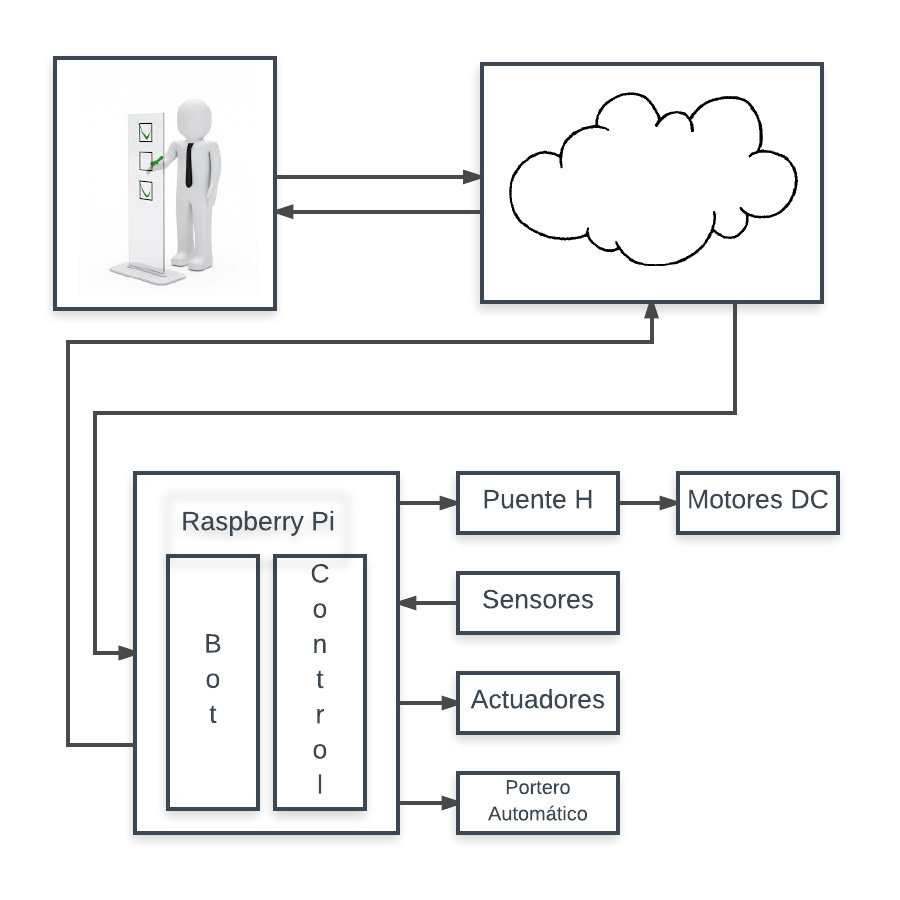
\includegraphics[scale=0.5]{ArqSist}
\caption{Arquitectura del sistema}
\label{fig:arqSist}
\end{figure}

En la figura \ref{fig:arqSist} se muestra la arquitectura del sistema que se va a desarrollar. 
Como vemos, el usuario no tiene contacto directo con el sistema. Pues aunque se encuentre la 
Raspberry Pi y el usuario en la misma red, la comunicación se estable con el servidor de telegram 
de por medio.

Una vez que el usuario envía un comando y el bot lo recibe, éste provoca un evento y envía 
la orden hacia la lógica de control. La cual actuará en consecuencia de su alrededor.

De igual forma que nosotros enviamos comandos al sistema, el sistema nos devolverá los diferentes 
datos que recoge por los sensores y servicios que se estén manejando en ese momento.

El componente principal del sistema será la Raspberry Pi, en concreto usaremos 
la versión 3. Se puede definir la Raspberry Pi como un ordenador de placa 
reducida. En su interior cuenta con un procesador ARM de 64bits con 4 núcleos a 
1,2GHz. Cuenta con 1GB de RAM, conectividad Wi-Fi y bluetooth.

Se puede decir que los demás componentes del sistema son genéricos, por lo que 
no dependemos de ningún componente concreto.

\section{Desarrollo Software}
Para el desarrollo del software, se va a utilizar NodeJS, para la comunicación con telegram se va a 
usar un módulo para interactuar con el API oficial de telegram. Este módulo nos proporciona los 
métodos y eventos principales a la hora de comunicarnos con el bot.

En base a los comandos que el usuario env, se va a desarrollar una máquina de estados que nos 
permitirá interactuar con nuestro sistema.

Las características que se van a incluir en nuestro sistema domótico son las siguientes:
\begin{itemize}
\item Control de usuarios: el acceso a los comandos de nuestro sistema queda restringido a 
usuarios autorizados. Se gestionarán dos tipos de permisos, administradores y usuarios.
\item Control de presencia: el sistema domótico mediante el protocolo ARP, puede saber los 
dispositivos que se encuentran en ese momento en la red. Teniendo en cuenta que según datos 
estadísticos el 51\% de la población mundial tiene un smartphone. Podemos tener constancia de 
quien se encuentra en casa y guardar un registro de entrada y salida.
\item Control remoto del portero automático: se dispondrá de una cámara en nuestra puerta la cual 
nos enviará una foto de quien se encuentra en ella cuando llamen al timbre. Pudiendo también enviar 
un mensaje de voz mediante Telegram y que este sea reproducido.
\item Control de temperatura: mediante el servicio online \textit{openweathermap}, obtendremos la 
temperatura en nuestra localización
\item Control de alarma: se desarrollará un sistema de alarma por control remoto, asistido en 
gran parte por nuestro sistema de control de presencia.
\item Control de sensores y actuadores: con los 18 GPIO de la Raspberry Pi se pueden combinar 
diferentes sensores y actuadores.
\end{itemize}

\subsection{API de Telegram}
Telegram ofrece dos tipos de API. La \textit{Telegram API}, que permite crear tu propio cliente 
telegram y la \textit{API Bot}, que permite crear programas dentro de la interfaz de un 
cliente de telegram. En el caso que a nosotros nos corresponde nos vamos a 
centrar en la \textit{API Bot}. 

Estos bots son aplicaciones de terceros que corren dentro de un cliente de 
telegram. Los usuarios podrán interactuar con estas aplicaciones mediante 
mensajes, comandos, envío de ficheros, mensajes de voz, etc. Que serán 
interpretados por nuestras aplicación.

\subsubsection{¿Qué se puede hacer con los bots?}
Los bots ofrecen diferentes posibilidades, por lo que vamos a enumerar algunas 
de ellas:
\begin{itemize}
  \item \textbf{Notificación de noticias.} Un bot puede interactuar con el 
  usuario enviando publicaciones de interés tan pronto como estas sean 
  publicadas.
  \item \textbf{Integrar Telegram con otros servicios.} Estos bots pueden 
  incluirse en un chat y hacer peticiones a servicios externos, como por 
  ejemplo: Github, Wikipedia, Youtube, IMDB.
  \item \textbf{Juegos.} Se puede integrar contenido en HTML5, para de esta 
  forma incluir juegos.
  \item \textbf{Crear herramientas.} Herramientas para usar tanto en chats como 
  de forma individual, como por ejemplo: predicciones meteorológicas, 
  traducciones, bots para votar, etc.
\end{itemize}

\subsubsection{¿Como funcionan los bots?}
Los usuarios pueden interactuar con los bots de dos formas diferentes:
\begin{itemize}
  \item Tratandolo como un \textit{usuario}, podemos abrir un chat con él o agregarlo a un grupo de tal
  forma que estará siempre escuchando y respoderá sólo cuando se introduzca un comando registrado.
  \item Ejecutandolo como una acción sobre el teclado, tan sólo tendremos que 
  introducir @botname seguido de la consulta, esto permite usar el bot en 
  cualquier chat o grupo sin necesidad de añadirlo.
\end{itemize}

Todos los mensajes, comandos y solicitudes enviados por el usuario pasan 
directamente a la aplicación en ejecución por el usuario. El servidor de 
Telegram se encarga del cifrado y la comunicación. La aplicación se comunica con 
el servidor de Telegram con un sencilla interface HTTPS, que es el llamado \textit{API 
Bot}.

En este punto se pueden distinguir dos procesos diferentes, el envío de mensajes 
del usuario al bot y el envío de mensajes desde el bot al usuario.

\subsubsection{Mensajes del usuario al bot}
Este tipo de mensajes que nosotros vamos a recibir en nuestra aplicación, son 
representados por un objeto JSON. Este objeto tiene 2 campos principales, cada uno representado por
un nuevo objeto JSON:
\begin{itemize}
  \item User. Este objeto contiene los datos del usuario envía el mensaje.
 Podemos ver los campos más relevantes en la tabla \ref{tab:User}
  
  \begin{table}[h]
  \centering
  \begin{tabular}{cc}
  id  & Identificador único de usuario \\ \hline
  first\_name & Nombre de usuario \\ \hline
  last\_name & Apellido del usuario \\ \hline
  username & Alias único del usuario \\ \hline
  \end{tabular} 
  \caption{User}
  \label{tab:User}
  \end{table}

  \item Chat. Este objeto contiene los datos del chat desde el que se envía el 
  mensaje. Podemos ver los campos más relevantes en la tabla \ref{tab:Chat}
  
   \begin{table}[h]
  \centering
  \begin{tabular}{>{\centering\arraybackslash}m{1cm} >{\centering\arraybackslash}m{4cm}}
  id  & Identificador único de usuario \\ \hline
  type & Tipo de chat, puede ser “private”, “group”, “supergroup” or “channel” 
  \\ \hline
  title & Título del chat \\ \hline
  \end{tabular} 
  \caption{Chat}
  \label{tab:Chat}
  \end{table}
  
  \item Message. En este objeto encontramos todos los campos referentes al 
  mensaje. Podemos ver los campos más relevantes en la tabla \ref{tab:Message}
  
   \begin{table}[h]
  \centering
  \begin{tabular}{>{\centering\arraybackslash}m{1cm} >{\centering\arraybackslash}m{4cm}}
  message\_id  & Identificador del mensaje \\ \hline
  from & Identificador del emisor, vacío si viene de un chat \\ \hline
  date & Fecha del mensaje \\ \hline
  text & Texto recibido en el mensaje \\ \hline
  audio & Información sobre el archivo. \\ \hline
  document & Información sobre el archivo \\ \hline
  voice & Información sobre el archivo \\ \hline
  photo & Información sobre el archivo \\ \hline
  \end{tabular} 
  \caption{Message}
  \label{tab:Message}
  \end{table}

\end{itemize}
Los campos que no contengan información relevante no serán recibidos.

\subsubsection{Mensajes del bot al usuario}
Al igual que el usuario puede enviar al bot mensajes de texto, audios, mensajes 
de voz, fotos, etc. el bot puede hacer lo propio hacia los usuarios. La única 
información necesaria en este caso es el id del usuario.
Por ejemplo, para enviar un audio, usaremos el método \textit{sendAudio()}, como 
argumentos a este método le pasaremos el ID del usuario y la ruta al fichero de 
audio que se va a enviar.


\subsection{Máquina de estados}
En la figura \ref{fig:MaqEstPrin} se puede ver el diagrama de flujo de la primera toma de decisiones. 
\begin{figure}[h]
\centering
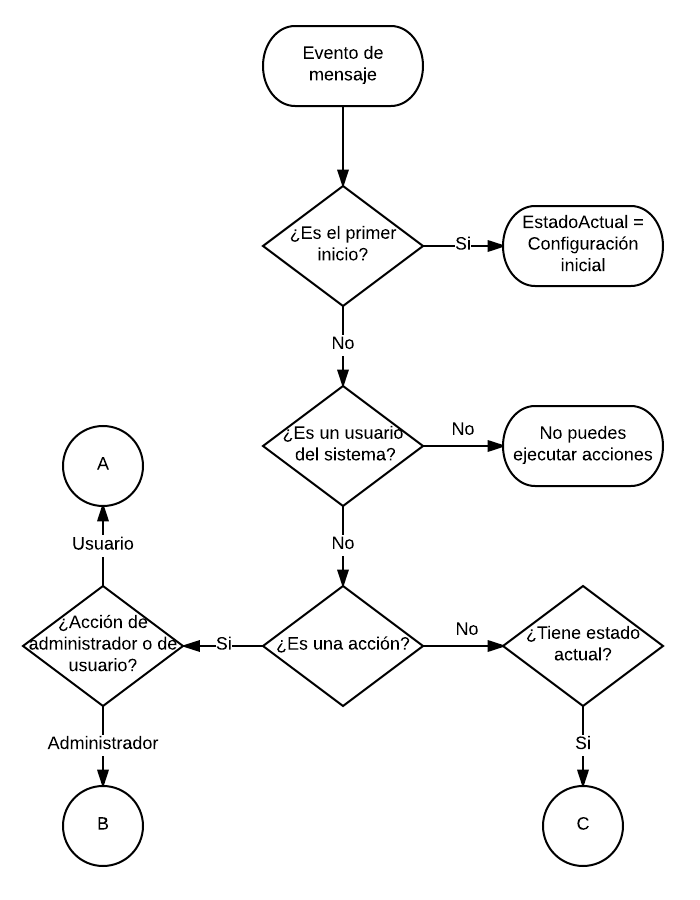
\includegraphics[scale=0.5]{MaqEstPrin}
\caption{Máquina de estados Principal}
\label{fig:MaqEstPrin}
\end{figure}

Cuando nosotros enviamos un mensaje a nuestro control, la primera premisa que tenemos es 
ser usuario del sistema, si esto no se cumple directamente seremos expulsados.
Si somos usuarios del sistema, se evaluará si hemos enviado una acción o un mensaje, en el 
caso de ser una acción esta será evaluada como una acción de usuario o de administrador tal y 
como podemos ver en las figura \ref{fig:MaqEstAcc}, si no coincide con ninguna de ellas se 
enviará un mensaje de error.

Además de estas acciones, existe una acción especial \textit{/help}, que le muestra al usuario 
todas las acciones que tiene disponible.

\begin{figure}[h]
\centering
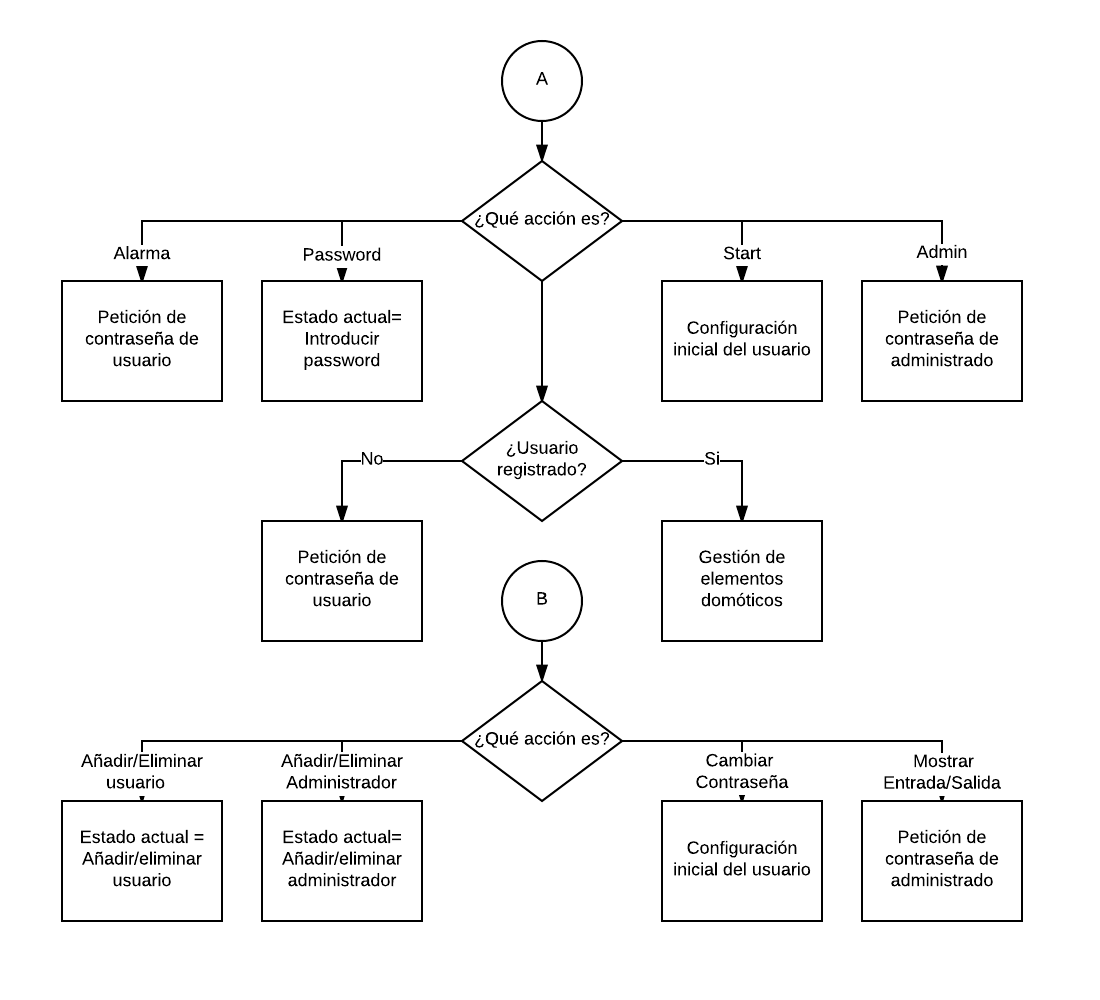
\includegraphics[scale=0.4]{MaqEstAcc}
\caption{Máquina de estados Acciones}
\label{fig:MaqEstAcc}
\end{figure}

En el caso de que no sea una acción, se evaluará si el controlador está esperando una respuesta 
de nosotros a una acción anterior. Este proceso forma una nueva máquina de estados que estará 
controlada por la variable \textit{"estado actual"}, que es independiente para cada usuario.
Este tratamiento lo veremos con más detalle en la subsección \ref{sec:ControlUsuarios}

\subsection{Control de usuarios}\label{sec:ControlUsuarios}

A continuación, vamos a ver como se gestionan los diferentes usuarios del sistema y cuales 
son las posibilidades que tiene cada tipo de usuario.

Cada usuario en telegram se identifica por un ID único que se asigna automáticamente en 
el momento del registro en la aplicación y además por un alias, también único, el cual se asigna el 
propio usuario. Nuestro API puede usar los dos identificadores para enviar los  mensajes, sin embargo, 
hemos optado por realizar el envío de de los mensajes siempre a través del ID, pues de esta forma 
tenemos la certeza de que nunca va a fallar el envío del mensaje. 

Los usuarios se almacenan en una variable \textit{users}, identificando a cada usuario por su alias.

\begin{figure}[h]
\centering
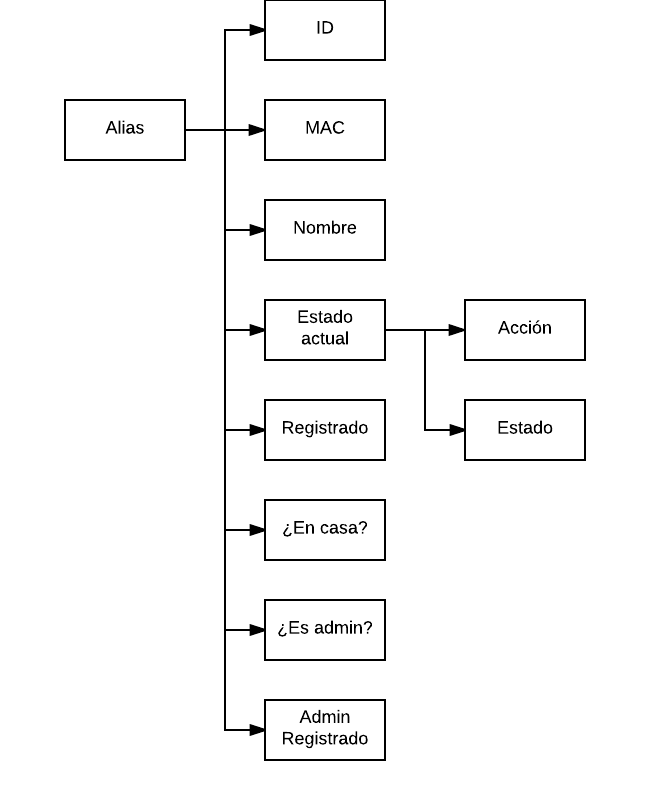
\includegraphics[scale=0.5]{UserEst}
\caption{Estructura de usuario}
\label{fig:UserEst}
\end{figure}

La estructura de  usuario se puede ver en la fig. \ref{fig:UserEst}. A continuación se va a explicar 
el significado y el uso de cada propiedad:
\begin{itemize}
\item Alias: es el nombre con el que se identificarán a los usuarios. Cuando el bot recibe un mensaje 
de un usuario, recibimos su alias como identificación.
\item ID: número de identificación, que se usará para enviar mensajes a este usuario cuando sea 
necesario, al igual que el alias lo recibimos en cada mensaje que envía el usuario.
\item MAC: aquí almacenaremos la MAC del teléfono del usuario. La MAC la se utilizará en el 
sistema de control de presencia y la obtendremos habilitando un servidor desde nuestra 
Raspberry Pi y pidiendole al usuario cuando se registre que acceda a ese servidor.
\item Registrado: cuando el usuario introduzca la contraseña de usuario del sistema, en 
este campo se introducirá la hora del registro, para controlar que cuando se cumpla el tiempo 
configurado por el administrador este usuario tenga que volver a introducir la contraseña.
\item ¿En casa?: esta propiedad indica si el usuario está en casa. 
\item ¿Es admin?: esta propiedad indica si el usuario es administrador.
\item Admin registrado: tiene la misma función que la propiedad \textit{registrado}, pero esta 
vez como administrador 
\item Estado actual: esta propiedad nos permite interactuar con el sistema continuamente, 
cuando se utilice una acción que necesite más información, la propiedad \textit{acción} toma 
el valor de la acción pedida y la propiedad \textit{estado} se irá actualizando dependiendo de 
la cantidad de datos que se necesiten.
\end{itemize}

Un apartado importante sobre el control domótico es la seguridad, no se puede permitir que 
una persona externa se conecte a nuestro sistema. El problema que se encuentra al introducir 
la contraseña es la imposibilidad de que se edite el mensaje automáticamente por el sistema, 
ya que telegram sólo ofrece la posibilidad de editar mensajes propios. 

\begin{figure}[h]
\centering
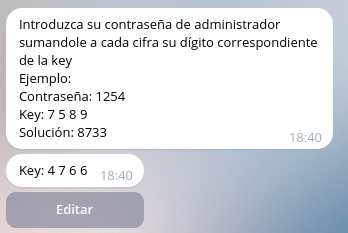
\includegraphics[scale=0.6]{imgPass}
\caption{Proceso introducción contraseña}
\label{fig:imgPass}
\end{figure}

Para subsanar este problema, el sistema generará una key aleatoria, la cual enviará con un 
botón de edición. El usuario deberá sumar esta key a la contraseña real término a término.
De esta forma, al pulsar el botón de \textit{Editar}, el sistema automáticamente eliminará el 
mensaje con la key, podemos ver el proceso en la figura \ref{fig:imgPass}

\textbf{AQUI AÑADIR UN DIAGRAMA DE ACTIVIDAD}

\subsection{Control de presencia}
Para la detección de presencia nos hemos basado en el protocolo ARP. Sabiendo la 
ínfima posibilidad que hay de coincidir dos MAC en un misma red, cada usuario 
será identificado en por el sistema con la MAC de su smartphone. De esta forma, 
cada vez que tengamos una conexión o desconexión en nuestra red se detectará el 
dispositivo y se asociará con un usuario.

Estas entradas y salidas se van a ir almacenando en un fichero CSV diario, a los 
cuales sólo los administradores del sistema tendrán acceso. 

La forma de detectar la MAC del usuario es mediante un servidor creado en 
nuestra red local, al cual el usuario deberá conectarse. Con este proceso el 
sistema obtendrá la IP del dispositivo del usuario. 
Cabe recordar que la comunicación con el sistema se realiza a través de la 
aplicación de mensajería, por lo tanto aunque nos encontremos en la misma red 
que el sistema no se podrá obtener la IP enviando un mensaje, pues la 
identificación que se utiliza en la aplicación de mensajería es diferente.

Una vez que eser tenga la IP del usuario, en el siguiente reconocimeinto que se 
haga de la red se identificará la MAC del usuario y se le asignará en su 
correspondiente entrada, como se vio en la subsección \ref{sec:ControlUsuarios}

\textbf{AÑADIR UN DIAGRAMA DE ACTIVIDAD}

\subsection{Control remoto del portero automático}
Mediante los mensajes de voz integrados en Telegram, un altavoz y una cámara se  
ha desarrollado este sistema para el control remoto del portero automático. 

Este control se activará cuando alguien llame al timbre, uno de los GPIO de la 
raspberry emitirá el evento que iniciará una captura de la cámara. Esta 
captura se enviará a cada usuario del sistema. 
Para poder responderle a quien llama, el usuario del sistema puede enviar un mensaje de voz mediante
telegram, este mensaje de voz se reproducirá por un altavoz instalado en el sistema.

Cuando un usuario de Telegram envía un mensaje de voz mediante la aplicación, 
este mensaje se almacena en su servidor, por lo que cuando recibamos el mensaje 
de voz en nuestra aplicación la información que obtendremos será el ID del 
fichero en el servidor. Por lo que una vez recibido este ID, tendremos que 
descargar el audio, mediante el método \textit{downloadFile} del API de 
Telegram.
El fichero descargado se encuentra en formato \textit{ogg} usando el codec 
\textit{opus}, este fichero no se puede reproducir directamente desde la 
terminal de linux. Por lo tanto, este fichero se convierte a formato un formato común como es 
el \textit{wav}, que será el que podamos reproducir.

\subsection{Control de sensores y actuadores}
Para el control de los sensores y los actuadores se van a usar log GPIOs de la 
Raspberry Pi, aunque tambien es posible encontrarlos controlados por USB.

Para el control de los GPIOs se usará el módulo de NodeJS llamado 
\textit{rpi-gpio}, con este módulo tenemos preparado los métodos para configurar 
los GPIO, escribir, leer y escuchar los eventos que producen los cambios.

Los sensores y actuadores a incluir dependerá de las peticiones del usuario, ya 
que los GPIOs son bastante polivalentes en cuanto a funcionalidad, por lo que se 
dejarán preparadas las funciones para trabajar con los siguientes elementos, 
aunque se podrían añadir más:

\begin{itemize}
  \item Luces: un funcionamiento sencillo como es el apagar y encender luces, a 
  petición del usuario el pin configurado para esta función se pondrá al valor 
  pedido.
  \item Climatización: al igual que con las luces, se puede preparar la 
  climatización para ser encendida y apagada.
  \item Toldos y persianas: este control se podría simular con motores DC, estos 
  motores regulan su velocidad mediante PWM y se controla la posición inicial y 
  final mediante finales de carrera. 
  Por consiguiente, midiendo el tiempo entre la 
  posición final y la inicial se puede hacer aproximaciones de posiciones 
  intermedias. La velocidad de subida y bajada será fija.
\end{itemize}

\subsection{Control de temperatura}
El control de la temperatura se va a realizar mediante el API del servicio online openweathermap, 
Cada hora se ejecutará un método en nuestro sistema que hará una petición al 
servicio de openweathermap, cuando se realice esta petición, dependiendo de la 
configuración de los sensores y actuadores se realizarán una serie de 
evaluaciones para ajustar nuestro hogar a las condiciones meteorológicas y a la 
temperatura del momento.

Nuestro sistema necesita tener las coordenadas de su ubicación, así que cuando 
se realice la configuración inicial del bot nos pedirá que enviemos la ubicación 
en la que se encuentra. Esto se realizará mediante las opciones de telegram, el 
sistema recibirá la ubicación y almacenará las coordenadas de estas.

\subsection{Control de alarma}
La alarma contará con sensores de apertura de puertas y ventanas para la 
detección y una señal acústica para indicar la presencia dentro del hogar.

El proceso de activar y desactivar la alarma será siempre manual, aunque el 
sistema de detección de presencia servirá de asistente, de forma que cuando no 
haya nadie en casa enviará a todos los administradores un mensaje avisando de la 
desprotección del hogar. 

Todos los usuarios tienen permisos para activar y desactivar la alarma, pero 
aunque estén registrados tendrá que insertar la contraseña para que la acción 
tenga efecto. De esta forma, una vez que el sistema detecte presencia, en la 
entrada, dará al usuario un margen de 15 segundos para desactivar la alarma.

\subsection{Almacenaniento de opciones}
En este apartado, vamos a ver como se almacenan las opciones de forma permanente a la 
espera para prevenir la pérdida de datos con la caida de la aplicación. La cantidad de 
información que se maneja no tiene tamaño como para usar una base de datos como 
mySQL, MongoDB, etc. 
Se ha optado por almacenar los datos persistentes en archivos CSV, de esta forma 
tenemos implementado un módulo de lectura y escritura de este tipo de archivos para 
en un futuro poder usar el envío de ficheros CSV para configurar el sistema, añadir usuarios, etc.

\section{Pruebas de Rendimiento}
Se han realizado pruebas de rendimiento en los siguientes componentes del sistema:
\begin{itemize}
  \item Respuesta al protocolo ARP
  \item Captura de foto
  \item Proceso de recepción y reproducción de audio
  \item Petición y tratamiento de datos meteorlógicos
\end{itemize}
 la respuesta al protocolo ARP, captura de una foto y el proceso de envío de 
un audio. Estas pruebas de rendimientos se van a realizar sobre diferentes 
plataformas como son:
\begin{itemize}
\item Raspberry Pi B+
\item Raspberry Pi 3
\item SSOO Debian virtualizado sobre MacBook Pro
\end{itemize}

\subsection{Respuesta protocolo ARP}

\subsection{Captura de foto}

\subsection{Proceso de recepción y reproducción de audio}

\subsection{Petición y tratamiento de datos meteorológicos}


\section{Costes}
El tiempo desarrollo de este sistema domótico ha sido de 300 horas, tomando un 
precio por hora de 30\euro, tenemos un coste de desarrollo de 9000\euro.

Luego cada sistema tendría un coste fijo de:
\begin{table}[h]
\centering
\begin{tabular}{ccc}
Raspberry Pi & ........ & 60\euro \\
Sensores Alarma & ........ & 10\euro \\
Cámara & ........ & 15\euro \\
Altavoz & ........ & 10\euro \\
\hline \\
Total & ........ & 95\euro \\
\end{tabular} 
\caption{Costes fijos}
\label{tab:CostesFij}
\end{table}

Para cubrir los costes con la venta de 100 terminales, cada terminal debería tener un precio de 
185\euro (IVA no incl.)
A estos costes habría que sumarle los sensores y actuadores que desea el cliente y el coste 
de su instalación.

\section{Conclusiones}
Durante el desarrollo del TFM, se ha podido ver como todos los objetivos 
planteados se han podido satisfacer positivamente.

En primer lugar, se ha podido ver como la Raspberry Pi, aunque con sus 
limitaciones cumple perfectamente con las exigencias que se pedian.

Con respecto al desarrollo del software mediante NodeJS, se ha podido ver como 
ha cumplido perfectamente con lo que esperabamos de él. La gran cantidad de 
módulos que se pueden encontrar desarrollados por la comunidad han facilitado el 
trabajo enormemente.

El último objetivo que nos planteamos fue que el sistema se controlara mediante 
una aplicación de mensajería. Se ha elegido Telegram, la cual hemos visto el API 
que ofrece para crear aplicaciones dentro de su cliente. Este API en conjunto 
con uno de los módulos de NodeJS nos ha permitido desarrollar nuestra aplicación 
sin dificultad pudiendo ofrecer todas las opciones que se deseaban.

\hfill mds
 
\hfill August 26, 2015

\begin{thebibliography}{1}

\bibitem{IEEEhowto:kopka}
H.~Kopka and P.~W. Daly, \emph{A Guide to {\LaTeX}}, 3rd~ed.\hskip 1em plus
  0.5em minus 0.4em\relax Harlow, England: Addison-Wesley, 1999.

\end{thebibliography}
\end{document}